% The coboundary delta of the 0-cochain: value 1 flows out along each
% incident 1-simplex (a red one reversed, so its value is -1).
% Source: book/tex/homology/cohomology.tex (§ Visualization of cohomology groups).
\documentclass[border=2mm]{standalone}
\usepackage{tikz}
\usepackage{amssymb}
\usetikzlibrary{arrows.meta,calc}
\begin{document}
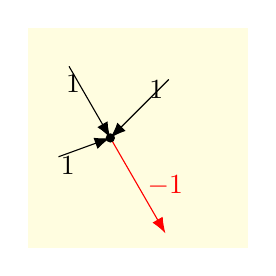
\begin{tikzpicture}[scale=0.7, >={Latex[length=2mm]}]
  \fill[yellow!12] (0,0) rectangle (4,4);
  \coordinate (A) at (1.5,2);
  \draw[->] ($(A)+(45:1.5)$) -- (A) node[midway, above right] {$1$};
  \draw[->] ($(A)+(120:1.5)$) -- (A) node[midway, above left] {$1$};
  \draw[->] ($(A)+(200:1)$) -- (A) node[midway, below left] {$1$};
  \draw[red, ->] (A) -- ($(A)+(-60:2)$) node[midway, right] {$-1$};
  \fill (A) circle (2.4pt);
\end{tikzpicture}
\end{document}
